Приложение реализовано на языке Python с использованием библиотек Panda3d и NetworkX. Поддерживается загрузка конфигурации спутниковой группировки и терминалов. Пример конфигурации:

\begin{verbatim}
{
    "camera_rotation_angle": 0,
    "camera_rotation_angle_vertical": 0,
    "camera_radius": 40,
    "dash_cone_angle": 65,
    "time_factor": 500.0,
    "update_topology_interval": 0.1,
    "sending_interval": 0.05,
    "loss_probability": 0.2,
    "window_size": 8,
    "timeout": 0.5,
    "sprite_size": 0.5,
    "num_orbit_segments": 1000,
    "orbit_color": [1, 1, 1, 0.8],
    "orbit_thickness": 1.5,
    "path_color": [0, 1, 0, 0.8],
    "path_thickness": 1.5,
    "dashes": [
        {
            "lat": 56.85,
            "long": 60.61
        },
        {
            "lat": 40.42,
            "long": -74.00
        }
    ],
    "satellites": [
        {
                "a": 26.6,
                "e": 0.74,
                "i": 63.4,
                "omega": 0,
                "w": 90,
                "m": 270
        },
        {
                "a": 26.6,
                "e": 0.74,
                "i": 63.4,
                "omega": 90,
                "w": 90,
                "m": 90
        }
    ]
}
\end{verbatim}
\newpage
Управление началом передачи осуществляется через форму.

\begin{figure}[H]
    \centering
    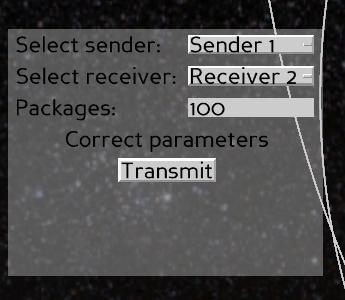
\includegraphics[width=0.5\linewidth]{form.png}
    \caption{Форма управления}
    \label{fig:form}
\end{figure}

Терминалы отображаются в виде ''спутниковой тарелки'', спутники в виде соответствующего значка.

\begin{figure}[H]
    \centering
    
\includegraphics[width=0.25\linewidth]{satellite-dash.png}
    \caption{Обозначение терминала}
    \label{fig:dash}
\end{figure}

\begin{figure}[H]
    \centering
    
\includegraphics[width=0.25\linewidth]{satellite.png}
    \caption{Обозначение спутника}
    \label{fig:satellite}
\end{figure}

Вращение камеры осуществляется мышью. При передаче данных путь передачи отображается зеленой линией.